%! Suppress = Unicode
\documentclass[a4paper,UKenglish,cleveref, autoref]{templates/lipics-v2019}
\usepackage{csquotes}
\usepackage{url}
\usepackage{pgfplots}
\usepackage{pgf-pie}
\usepackage{float}
%This is a template for producing LIPIcs articles.
%See lipics-manual.pdf for further information.
%for A4 paper format use option "a4paper", for US-letter use option "letterpaper"
%for british hyphenation rules use option "UKenglish", for american hyphenation rules use option "USenglish"
%for section-numbered lemmas etc., use "numberwithinsect"
%for enabling cleveref support, use "cleveref"
%for enabling cleveref support, use "autoref"

\newcommand{\sls}{Safer Language Subset}
\newcommand{\slss}{Safer Language Subsets}

\newcommand{\sqs}{Software-Qualitätsstandard}
\newcommand{\sqss}{Software-Qualitätsstandards}

\newcommand{\misra}{MISRA-C}

\graphicspath{{./graphics/}}%helpful if your graphic files are in another directory

\bibliographystyle{plainurl}% the mandatory bibstyle

\title{M10: \sqss}

\titlerunning{M10: \sqss}%optional, please use if title is longer than one line

\author{Alexander Linder}{Karlsruhe Institute of Technology, Germany \and \url{https://kit.edu} }{alexander.linder@student.kit.edu}{}{}
%mandatory, please use full name; first two parameters are mandatory, other parameters can be empty.

\authorrunning{A. Linder}
%mandatory. First: Use abbreviated first/middle names. Second (only in severe cases): Use first author plus 'et al.'

\Copyright{Alexander Linder}
%%mandatory, please use full first names. LIPIcs license is "CC-BY";  http://creativecommons.org/licenses/by/3.0/

\ccsdesc[100]{Software and its engineering~Software reliability}
%mandatory: Please choose ACM 2012 classifications from https://dl.acm.org/ccs/ccs_flat.cfm

\keywords{\misra, \sqss}
%mandatory; please add comma-separated list of keywords

\category{}
%optional, e.g. invited paper

\relatedversion{}
%optional, e.g. full version hosted on arXiv, HAL, or other respository/website

\supplement{}
%optional, e.g. related research data, source code, ... hosted on a repository like zenodo, figshare, GitHub, ...

\funding{}
%optional, to capture a funding statement, which applies to all authors. Please enter author specific funding statements as fifth argument of the \author macro.

\acknowledgements{}
%optional

\nolinenumbers %uncomment to disable line numbering

\hideLIPIcs  %uncomment to remove references to LIPIcs series (logo, DOI, ...), e.g. when preparing a pre-final version to be uploaded to arXiv or another public repository

\lstset{language=C,
    basicstyle=\ttfamily,
    keywordstyle=\color{blue}\ttfamily,
    stringstyle=\color{red}\ttfamily,
    commentstyle=\color{gray}\ttfamily,
    morecomment=[l][\color{gray}]{\#}
}

%Editor-only macros:: begin (do not touch as author)%%%%%%%%%%%%%%%%%%%%%%%%%%%%%%%%%%
\EventEditors{}
\EventNoEds{0}
\EventLongTitle{Proseminar Werkzeuge und Methoden der Software-Analyse}
\EventShortTitle{Proseminar}
\EventAcronym{Proseminar}
\EventYear{2019}
\EventDate{WS19/20}
\EventLocation{Karlsruhe, Deutschland}
\EventLogo{}
\SeriesVolume{}
\ArticleNo{M10}
%%%%%%%%%%%%%%%%%%%%%%%%%%%%%%%%%%%%%%%%%%%%%%%%%%%%%%

\begin{document}

    \maketitle

    \begin{abstract}
        Diese Arbeit gibt einen Überblick über \sqss\ im Allgemeinen, unter besonderer Betrachtung eines weitverbreiteten Beispiels: \misra\ 2004.\\
        Es wird die hinter \sqss\ stehende Motivation dargebracht, sowie betrachtet, wie sich Regeln innerhalb eines Standards sinnvoll klassifizieren lassen.
        Dies führt zum Begriff des \slss\ nach Hatton, welches formale Forderungen an einen guten Regelsatz aufstellt.
        Weiterhin wird überprüft, inwiefern \misra\ diese Definition erfüllt.\\
        Final sollen Gütekriterien für \sqss\ aufgestellt und die Güte des \misra\ Standards unter eben diesen Kriterien bewertet werden.
        Hierbei wird insbesondere die Signal-Rausch-Rate des Standards näher betrachtet.\\
        Die Arbeit kommt zum Schluss dass \misra\ selbst einige Schwächen besitzt, welche durch sinnvolles Subsetting
        ausgeglichen werden können.
    \end{abstract}

    \section{Einleitung}
    \label{sec:einleitung}
    \sqss\ finden weite Verbreitung in der Industrie.
    Doch warum ist das so?
    Übergeordnetes Ziel von \sqss\ ist das Schaffen eines einheitlichen Programmierstils innerhalb einer Firma bzw.\ eines
    Projektteams.
    Damit soll die Programmiersprache, in den meisten Fällen C oder C++, auf sichere Features beschränkt werden, was den
    Code leichter wartbar machen und final für mehr Codequalität und weniger Fehler sorgen soll.\\
    Ein gutes Beispiel für solch ein unsicheres Sprachfeature ist die Operatorpräzedenz in C, sowie den von ihr beeinflussten
    Sprachen.
    C besitzt wie auch die Mathematik eine recht große Menge an Operatoren.
    Diese beiden Mengen unterscheiden sich jedoch in einem kleinen, aber feinen Punkt.
    In der Mathematik wird bis auf die grundlegendsten Präzedenzen wie Punkt vor Strich nur sehr wenig mit Präzedenzregeln
    gearbeitet.
    Im Allgemeinen müssen Klammern gesetzt werden.
    Dies ist in C-artigen Sprachen nicht so.
    C bspw.\ besitzt eine Operatorpräzedenztabelle mit insgesamt 15 Prioritätsstufen, um lästiges Klammerschreiben vermeidbar
    zu machen.
    Bei diesen Prioritäten handelt es sich jedoch um eine bekannte und nicht zu unterschätzende Fehlerquelle.\\
    Beispiele für \sqss\ sind der JSF AV (Joint Strike Fighter Air Vehicle) Standard für C++, der von Lockheed Martin
    für den namensgebenden Joint Strike Fighter verwendet wurde und frei im Netz verfügbar ist, der CERT C Coding
    Standard des CERT Coordination Centers oder \misra, einer der weitverbreitetsten Standards, vorallem in der
    Automobilindustrie.\\
    Wir wollen im Folgenden \sqss\ im Allgemeinen näher betrachten und am Beispiel \misra\ sinnvolle Klassifikationen
    von Regeln sowie mögliche Gütekriterien und -Analysen für Standards vorstellen.

    \section{\misra}
    \label{sec:misra-c}
    \misra\ ist ein weitverbreiteter \sqs,
    der von der \textbf{M}otor \textbf{I}ndustry \textbf{S}oftware \textbf{R}eliability \textbf{A}ssociation (MISRA) entwickelt wurde.
    Die erste Version von \misra\ wurde 1998 veröffentlicht, mit insgesamt zwei großen Revisionen einmal 2004 sowie 2012,
    wobei sich diese Arbeit auf die Standards von 1998 (künftig M1998) und 2004 (künftig M2004) beschränkt,
    da einerseits der Standard von 2004 nach wie vor weite Verbreitung findet und sich andererseits die Forschung
    auf diese beiden Versionen konzentriert.\\
    Bei \misra\ handelt es sich nach~\cite{misra-website} um den de facto Standard zur Programmierung eingebetteter Systeme
    in der Mehrheit der sicherheitsrelevanten Industrien in der Programmiersprache C\@.
    Verbreitung findet \misra\ dabei überwiegend in der Automobilindustrie, wird jedoch auch von Bahn, Luftfahrt, Militär
    sowie dem medizinischen Sektor genutzt.\\
    Sowohl M1998 als auch M2004 nehmen Bezug auf C89/90 und nicht auf den neueren C-Standard C99 (ISO/IEC9899:1999),
    was dazu führt, dass neuere Sprachkonstrukte in \misra-konformem Code nicht erlaubt sind,
    auch wenn die verwendeten Compiler sie unterstützen.

    \subsection{Evolution des Standards}
    \label{subsec:evolution-des-standards}
    Die Revision von M1998 auf M2004 verfolgte im Großen und Ganzen fünf Ziele:

    \begin{itemize}
        \item Die Übereinstimmung der verwendeten Begriffe mit denen des C-Standards sicherzustellen
        \item Allgemeine Regeln zu undefiniertem Verhalten durch Spezialisierte zu ersetzen
        \item Das \enquote{Eine Regel, ein Fehler}-Prinzip durchzusetzen.
            (Komplexe Regeln in atomarere aufzuspalten)
        \item Neue und verbesserte Codebeispiele hinzuzufügen
        \item Manuelle Verwendung (ohne Analysetools) zu entfernen
    \end{itemize}

    Um diese Ziele zu erreichen wurde unter anderem an der Anzahl und der Verteilung der Regeln in die beiden Kategorien
    \enquote{Empfohlene} und \enquote{Verpflichtende} gearbeitet.
    In Figure~\ref{fig:bar-1998-2004} ist die absolute Verteilung von Regeln in die beiden Kategorien aufgetragen.
    Im dritten Balkenpaar sind weiterhin die Gesamtanzahlen der Regeln aufgetragen.
    In Figure~\ref{fig:pie-1998-2004} lassen sich die prozentualen Anteile der beiden Regelkategorien ablesen.

    \begin{figure}[H]
        \centering
        \captionsetup{justification=centering,margin=2cm}
        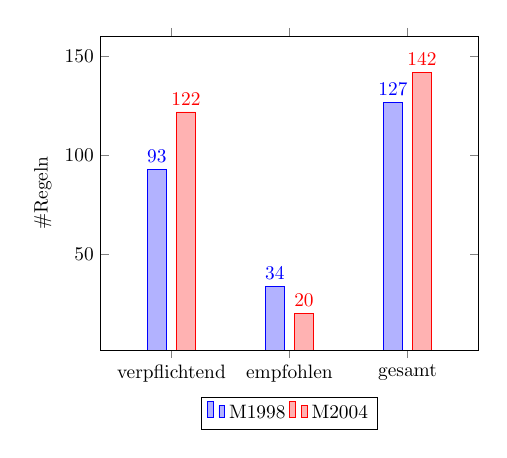
\begin{tikzpicture}[scale=0.7]
    \begin{axis}[
    ybar,
    enlarge x limits=0.30,
    enlarge y limits=0.15,
    legend style={at={(0.5,-0.15)},
    anchor=north,legend columns=-1},
    ybar=5pt,% configures `bar shift'
    ylabel={\#Regeln},
    symbolic x coords={verpflichtend,empfohlen,gesamt},
    xtick=data,
    nodes near coords,
    ]
        \addplot coordinates {(verpflichtend,93) (empfohlen,34) (gesamt,127)};
        \addplot coordinates {(verpflichtend,122) (empfohlen,20) (gesamt,142)};
        \legend{M1998,M2004}
    \end{axis}
\end{tikzpicture}
        \caption{Regelanzahl 1998 vs 2004}
        \label{fig:bar-1998-2004}
    \end{figure}

    \begin{figure}[H]
        \centering
        \captionsetup{justification=centering,margin=2cm}
        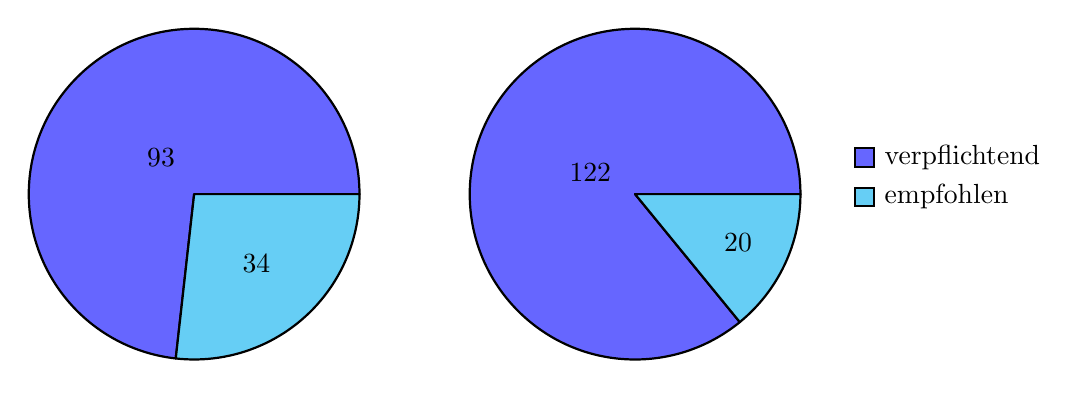
\begin{tikzpicture}[scale=0.7]
    \pie[sum=auto]{93/ , 34/ }
    \pie[pos={8,0},sum=auto, text=legend]{122/verpflichtend, 20/empfohlen}
\end{tikzpicture}
        \caption{Regelanteile 1998 vs 2004}
        \label{fig:pie-1998-2004}
    \end{figure}

    Wie man anhand der Grafiken erkennen kann, hat sich die Anzahl der Regeln in M2004 insgesamt erhöht und der Anteil
    der verpflichtenden Regeln ist gestiegen.
    Dies geht einher mit dem Ziel, große Regeln in mehrere kleinere aufzuteilen um diese leichter zu entscheiden
    und verständlich zu machen, sowie den Fokus auf die verpflichtenden, also die \enquote{essentielleren} Regeln zu verschieben.
    Teilweise ist den Machern des Standards dies gelungen, jedoch gibt es nach wie vor viele lange und komplexe Regeln.
    Wir wollen ein repräsentatives Beispiel auszugsweise näher betrachten:

    \subsection{Beispielregel}
    \label{subsec:beispielregel}

    Die folgende Beispielregel ist aus \misra\ unverändert (ausgenommen des Stylings) übernommen.
    Wir wollen an dieser möglichst möglichst kurzen, aber dennoch repräsentativen Regel die Formulierung des Regelsatzes
    analysieren und bewerten, inwiefern diese dem Ziel eines möglichst einfachen, leicht umsetzbaren Standards zuträglich ist.\\

    \noindent
    \begin{minipage}{\linewidth}
        \begin{example}
            \textbf{Rule 2.1 (required): Assembly language shall be encapsulated and isolated\cite{MISRA2004}}\\
            Where assembly language instructions are required it is recommended that they be encapsulated
            and isolated in either (a) assembler functions, (b) C functions or (c) macros.\\
            For reasons of efficiency it is sometimes necessary to embed simple assembly language instructions
            in-line, for example to enable and disable interrupts.
            If it is necessary to do this for any reason, then it is recommended that it be achieved by using macros.\\
            Note that the use of in-line assembly language is an extension to standard C, and therefore also
            requires a deviation against Rule 1.1.
            \begin{lstlisting}[language=C]
                #define NOP asm(" NOP")
            \end{lstlisting}
        \end{example}
    \end{minipage}

    Die Regel beschreibt wie Assemblerinstruktionen in den C-Code eingebettet werden sollen.
    Hierfür bestehen grundsätzlich drei Möglichkeiten, als Assemblerfunktionen, C Funktionen oder Makros.
    Soweit ist die Regel klar und sinnvoll aufgebaut.
    Im Nachfolgenden werden mögliche Abweichungen von der Regel erläutert.
    Unter anderem wann und wie die Verwendung von inline Assembler erlaubt ist und wie dies von statten gehen soll.
    Hier stellen sich gleich mehrere Fragen:

    \begin{itemize}
        \item Was genau ist eine \enquote{einfache} Assemblerinstruktion?
            Als Beispiel wird die (De-)Aktivierung von Interrupts genannt, doch wo soll allgemein die Grenze gesetzt werden?
        \item Es wird empfohlen inline Einbettungen mit Makros durchzuführen.
            Was ist zu tun wenn dies nicht über Makros geschieht.
            Verletzt das bereits die Regel oder ist es nur \enquote{unschön}?
    \end{itemize}

    Diese Fragen zeigen bereits auf, dass es alles andere als trivial ist, diese Regel automatisiert zu überprüfen.
    Angenommen, der Compiler überprüft sie für uns, wann setzt er die Grenze ab wann inline Assemblerinstruktionen
    nicht mehr \enquote{einfach} sind?
    Wird die Schwelle zu gering gesetzt, werden potentiell zu viele false positives erzeugt.
    Wird sie zu hoch gesetzt wird die Regel wertlos, da sie keine Ergebnisse mehr produziert.
    Beide Extreme sorgen dafür dass die Akzeptanz bei den Entwicklern sinkt, da sie im einen Fall störende false positives
    und im anderen Fall gar nie Fehler findet.
    Weiterhin erfordert inline Assembler eine Abweichung von Regel 1.1, was bedeutet dass für jede Inline-Instruktion,
    auch die, die durch diese Regel erlaubt werden, eine formale Abweichung von dieser Regel angegeben werden muss.\\
    Was folgt daraus?
    Die Regel lässt sich nur schwer sinnvoll automatisiert entscheiden und ist durch die vielen Ausnahmen und Überlappungen
    mit anderen Regeln komplex.
    Dies trifft auch auf viele andere Regeln in \misra\ zu, und ist eines der ersten Probleme des Standards, die auffallen
    und die sinnvolle Verwendung erschweren.

    \section{Regelklassifizierung}
    \label{sec:regelklassifizierung}
    In diesem Abschnitt wollen wir untersuchen, wie wir Regeln eines Regelsatzes sinnvoll klassifizieren können.
    Hierfür gibt es viele verschiedene Möglichkeiten.
    Im vorigen Abschnitt haben wir bereits gesehen, wie der Regelsatz von \misra\ organisiert wird.
    Hierbei handelte es sich schlicht um eine thematische Organisation der Regeln in Gruppen.
    Wir wollen nun eine alternative Klassifikationsart betrachten, die nicht auf dem Inhalt der Regeln, sondern auf ihrer
    Art sowie dem Grad an Evidenz, der ihre Existenz begründet, basiert.
    Regeln werden in diesem System nach Hatton in drei Typen unterschieden, einserseits Typ-A (\enquote{Style-basierte}) Regeln,
    andererseits Typ-B (\enquote{funktionale}) Regeln, welche sich weiter in Typ-B.1 (\enquote{Subjektive}) sowie
    Typ B.2 (\enquote{Evidente}) unterscheiden lassen.\cite{hatton2004safer}\\
    Im Folgenden wollen wir uns die verschiedenen Regelklassen je an einem Beispiel für eine Regel und ihre Verletzung
    genauer ansehen.\\
    Alle verwendeten Beispielregeln stammen hierbei aus \misra.

    \subsection{Typ-A Regeln}
    \label{subsec:typ-a-regeln}
    \begin{definition}
        Eine Typ-A Regel sei eine Regel, welche alleinig den Stil des Codes beeinflusst.
    \end{definition}

    Ein Beispiel für eine Typ-A Regel stellt Regel 5.7 \textit{No identifier name should be reused}
    (Kein Variablenname soll wiederverwendet werden) dar.\\
    Betrachten wir folgendes Code-Beispiel:

    \noindent
    \begin{minipage}{\linewidth}
        \begin{example}
            \lstinputlisting[title=\ ]{graphics/typa.c}
        \end{example}
    \end{minipage}

    Im Beispiel besitzen die Structs \textit{air\_speed} und \textit{gnd\_speed} je eine Membervariable \textit{speed}.
    Durch die unterschiedlichen Einheiten für Geschwindigkeit in der Luft bzw.\ am Boden besteht hier eine potentielle
    Fehlerquelle.
    Durch Umbenennung der Variablen in bspw.\ \textit{speed\_knots} und \textit{speed\_kmh} kann diese ausgeräumt werden,
    da klar wird, dass eine Konversion der Geschwindigkeiten stattfinden muss, bevor diese gemeinsam verwendet, bspw.\ verglichen,
    werden können.
    Ungeachtet dieser Fehlerquelle handelt es sich jedoch um ein rein stilistisches Problem, weshalb diese Regel in
    Kategorie A fällt.

    \subsection{Typ-B.1 Regeln}
    \label{subsec:typ-b-1-regeln}
    \begin{definition}
        Eine Typ-B.1 Regel sei eine Regel, welche potentiell unsichere Sprachfeatures ausschließt,
        jedoch keine empirischen Daten besitzt, die diesen Ausschluss begründen.
    \end{definition}

    Das klassische Beispiel schlechthin für eine Typ-B.1 Regel stellt Regel 14.4 \textit{The goto statement shall not be used}
    (Die goto Anweisung soll nicht verwendet werden) dar.
    Betrachten wir einmal folgendes Beispiel einer noch recht konservativen Verwendung des \textit{goto} rein zur
    Fehlerbehandlung:

    \noindent
    \begin{minipage}{\linewidth}
        \begin{example}
            \lstinputlisting[title=\ ]{graphics/typb1.c}
        \end{example}
    \end{minipage}

    Im Falle dass \textit{some Condition} eintritt, springt die Programmausführung zur Sprungmarke \textit{error}.
    Diese ist in einer \enquote{\textit{goto}-freien} Ausführung nicht erreichbar, da sie nach der ersten \textit{return}
    Anweisung steht.
    Wollen wir die Programmausführung analysieren müssen wir somit alle Verwendungen von \textit{goto} finden,
    um zu verstehen wann die \textit{error} Marke erreicht wird.
    \textit{Goto} erhöht damit die Komplexität von Programmen enorm, indem es die Lücke zwischen statischem
    Quelltext und darauf basierender Programmausführung vergrößert.\cite{goto-harmful}
    Eine empirische Datenbasis liefert uns diese Intuition nicht, dennoch enthält gemäß~\cite{hatton2004safer}
    nahezu jeder \sqs\ eine Regel dieser Form.\\
    Es handelte sich damit lange um \textit{das} Beispiel schlechthin für Typ-B.1 Regeln.
    Die von Hatton beschriebene klare Absenz von faktischer Untermauerung muss jedoch insofern in Frage gestellt werden,
    dass der Autor in~\cite{goto-study} eine Analyse der Auswirkung von \textit{goto} in Cobol-Programmen fand, die eine
    Korrelation der Nutzung von \textit{goto} mit geringerer Programmqualität nahelegt.
    Mit weiterer Faktenuntermauerung könnte unser Beispiel damit auch in die Kategorie B.2 wandern, die im Folgenden
    betrachtet wird.

    \subsection{Typ-B.2 Regeln}
    \label{subsec:typ-b-2-regeln}
    \begin{definition}
        Eine Typ-B.2 Regel sei eine Regel, welche potentiell unsichere Sprachfeatures ausschließt und empirische
        Daten besitzt, die diesen Ausschluss begründen.
    \end{definition}

    Typ-B.2 Regeln stellen damit sozusagen den \enquote{Goldstandard} für Regeln in einem \sqs\ dar.
    Sie sind weder rein stilistisch wie Typ-A Regeln, noch begründen sie sich auf Intuition wie Typ-B.1 Regeln.
    Betrachten wir im Folgenden die Regel 9.1 \textit{All automatic variables shall have been asigned a value before being used}
    (Alle lokalen Variablen müssen vor Benutzung initialisiert werden).\\
    Ein Beispiel:

    \noindent
    \begin{minipage}{\linewidth}
        \begin{example}
            \lstinputlisting[title=\ ]{graphics/typb2.c}
        \end{example}
    \end{minipage}

    Im dargestellten Listing wird eine Variable \textit{speed} deklariert, aber nicht initialisiert.
    Der erweiternde Erklärungstext in~\cite{MISRA2004} zu Regel 9.1 erlaubt eine spätere Initialisierung ausdrücklich, verlangt jedoch, dass
    in jedem Fall die Variable vor einem lesenden Zugriff beschrieben werden muss.
    Dies ist hier offensichtlich nicht der Fall, da \textit{speed} nur im Falle dass \textit{some Condition} eintritt auf
    \textit{101} gesetzt wird, andernfalls bleibt ihr Wert undefiniert.
    Damit ist ab dem lesenden Zugriff in der darauffolgenden If-Abfrage das Verhalten des Programms potentiell undefiniert.
    Es ist bereits intuitiv klar, warum es sich hierbei um eine Fehlerquelle handelt, jedoch gibt es hierzu auch explizit
    empirische Fehlerdaten, wie von Hatton dargelegt.\cite{hatton2004safer}

    \section{Safer Language Subsets}
    \label{sec:safer-language-subsets}

    Viele \sqss\ sind eine Ansammlung von Regeln der obigen Kategorien.
    Die meisten Standards versuchen diese Regeln weiter zu untergliedern, wie bspw.\ \misra\ in \textit{verpflichtende}
    und \textit{empfohlene} Regeln.
    Wir wollen im Folgenden ein \sls\ nach Hatton analog definieren.

    \begin{definition}
        Ein Regelsatz $R$ sei ein \sls $\iff$
        \begin{itemize}
            \item $R$ enthält nur Typ B.2 Regeln als verpflichtende Regeln
            \item $R$ enthält nur Typ B.1 Regeln als empfohlene Regeln
            \item $R$ enthält keinerlei Typ A Regeln
        \end{itemize}
    \end{definition}

    Diese Konstruktion eines \slss\ ermöglicht dem Standard auf \enquote{natürliche} Weise zu wachsen.
    Werden für eine Regel aus der Kategorie B.1 Fehlerdaten gefunden, so kann diese automatisch in die bessere Kategorie
    B.2 wandern, wie in Abschnitt~\ref{subsec:typ-b-1-regeln} mit der \textit{goto}-Regel angedeutet.\\
    In~\cite{hatton2004safer} begründet Hatton diese Definition damit, dass Mangel an begründenden Fehlerdaten eine der
    größten Barrieren ist, welche die Akzeptanz von Language Subsetting beeinträchtigt.
    Kennt ein Entwickler das mess- und quantifizierbare Risiko eines Sprachfeatures sei es besonders einfach, Ihn oder Sie
    davon zu überzeugen, das Feature nicht zu nutzen.
    Die Absenz solcher Fehlerdaten könnte jedoch als willkürliche Einflussnahme auf die Arbeitsweise des Entwicklers
    aufgefasst werden, was die Akzeptanz sinnvoller Maßnahmen senken könnte.
    
    \section{Bewertung}
    \label{sec:bewertung}

    %TODO Add introductory paragraph
    Nun wollen wir uns mit der Bewertung von \sqss\ und ihren Regeln beschäftigen.
    Hierbei gibt es nach~\cite{hatton2004safer} mehrere Kriterien, wovon wir einige nachfolgend näher beleuchten wollen:

    \subsection{Orthogonalität}
    \label{subsec:orthogonalität}
    Die Orthogonalität einer Regel $r$ bezeichnet den Grad der Unabhängigkeit von $r$ bezüglich der restlichen Regeln
    des Standards $S$.\\
    Weitergehende Analysen zur Orthogonalität würden den Rahmen dieser Arbeit sprengen, eine Analyse von M1998 findet sich
    jedoch in~\cite{hatton2004safer}.

    \subsection{Entscheidbarkeit}
    \label{subsec:entscheidbarkeit}
    Unter der Entscheidbarkeit einer Regel $r$ verstehen wir den Grad mit dem eine Überprüfung einer Regel auch wirklich das
    erreicht was sie soll.
    Damit eine Regel gut entscheidbar ist, muss diese alle möglichen zutreffenden Fälle vollständig spezifizieren und
    sollte möglichst keine Ausnahmen enthalten, welche false positives generieren könnten.\\
    Ein Beispiel für eine schlecht entscheidbare Regel stellt Regel 37 von M1998 dar, welche bitweise Operationen auf
    signed Integern verbietet.
    Die Regel lässt jedoch unspezifiziert, ob sie auf Fälle von Integer Promotion anzuwenden ist oder nicht.
    \footnote{Integer Promotion bezeichnet die implizite Konversion von Typen wie \textit{char} zu \textit{int} oder \textit{unsigned int}, sobald eine Operation auf ihnen ausgeführt wird.
    Ob \textit{int} oder \textit{unsigned int} verwendet wird hängt davon ab, ob ein \textit{int} alle Werte darstellen
    kann oder nicht.}

    \subsection{Atomizität}
    \label{subsec:atomizität}
    Manche Standards nutzen kurze, konzise Regeln, andere lange Prosaregeln.
    Eine Regel ist atomar, wenn sie nicht mit anderen Regeln überlappt und befolgt werden kann, ohne dass einzelne Teile der Regel gebrochen werden müssen.
    Weiterhin sollte eine Regel keine Ausnahmen besitzen, um als atomar bezeichnet werden zu können.\\
    Das Paradebeispiel einer nicht-atomaren Regel stellt Regel 1 dar, welche die Achtung des ISO C90 Standards fordert.

    \subsection{Signal-Rausch-Rate und False Positives}
    \label{subsec:signal-rausch-rate-und-false-positives}

    %TODO Explain what signal-noise-ratio means in context
    Unter der Signal-Rausch-Rate eines Standards verstehen wir die Rate mit der das Auftreten eines Verstoßes gegen den Regelsatz mit einem
    tatsächlichen Defekt korreliert.
    Großes Rauschen führt dazu, dass die Wahrscheinlichkeit dass ein Verstoß mit einem Defekt einhergeht, abnimmt.
    Ein Standard ist demnach \enquote{gut}, wenn die Signal-Rausch-Rate möglichst gering ist.\\
    Sei $p > 0$ sei die Wahrscheinlichkeit, mit der eine Korrektur einer Regelübertretung zur Einführung eines neuen Defekts
    etwa desselben Schweregrads führt.
    Diese Wahrscheinlichkeit existiert gemäß~\cite{transgression-data} und~\cite{hatton2007language} und beträgt in
    Adams Arbeit etwa den Wert $0,15$.\\
    Um nun die Relevanz von False Positives analysieren zu können betrachten wir die Rate $f$ mit der der Standard
    bei einer Regelübertretung auch einen Fault findet sowie die Rate $g$ mit der ein Verstoß einen False Positive, also
    einen Regelverstoß ohne assoziierten Fault, darstellt.
    Damit kann nun die gesamte Anzahl an Faults nach Korrektur aller Verstöße berechnet werden:
    \begin{lemma}
        Die gesamte Anzahl Faults nach Korrektur aller Regelverstöße gegen einen Standard berechnet sich als $fp + gp$
    \end{lemma}

    Da es zu Beginn jedoch bereits $f$ Faults gab, besteht die Möglichkeit dass ein stark rauschender Standard die Anzahl
    an Faults erhöht.
    Dies ist dann der Fall, wenn $fp + gp > f$ gilt.
    Dies lässt sich mittels Äquivalenzumformungen vereinfachen und führt damit zu:

    \begin{theorem}
        Die gesamte Anzahl Faults erhöht sich nach Korrektur aller Verstöße gegen einen Standard $\iff$
        \begin{gather*}
            \frac{f}{g} < \frac{p}{1-p}
        \end{gather*}
    \end{theorem}


    %TODO Explain graphics below
    In Figure~\ref{fig:1998-transgression-rates} und Figure~\ref{fig:2004-transgression-rates} werden anhand von sieben
    Softwarepaketen die kumulierten Verstöße je 1000 Codezeilen für M1998 bzw.\ M2004 je Regel dargestellt.
    Diese Untersuchung aus~\cite{hatton2007language} zeigt, dass mit der Einführung von M2004 die Rate der False Positives
    um lediglich $29\%$ gesunken ist.
    Damit folgt gemäß der Betrachtungen aus~\cite{hatton2007language} gemeinsam mit den Daten aus~\cite{transgression-data}
    dass M2004 noch immer in jenem Bereich liegt, in dem eine Korrektur aller Verstöße die Anzahl an Faults
    eher erhöht als verringert.\\
    Daraus muss geschlossen werden, dass Misra in seiner Reinform ungeeignet ist und eine sorgfältige Regelauswahl erfolgen
    muss um aus dem Standard einen Nutzen zu ziehen.

    \begin{figure}[H]
        \centering
        \captionsetup{justification=centering,margin=2cm}
        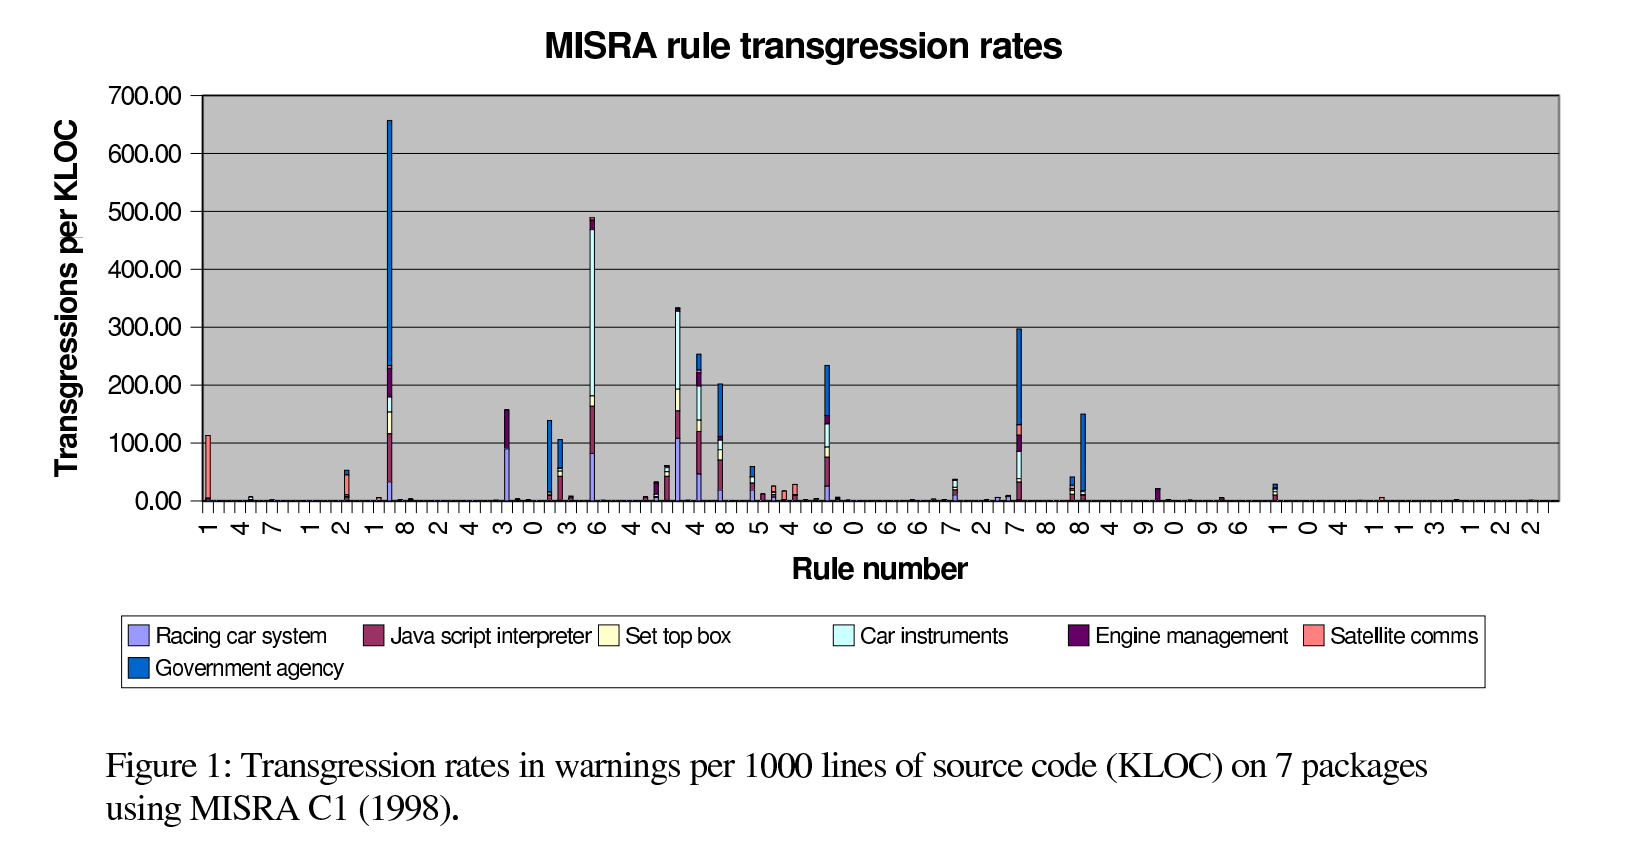
\includegraphics[width=\textwidth]{graphics/1998-transgression-rates.png}
        \caption{Verstöße in Warnungen je 1000 Codezeilen auf 7 Pakete verteilt, M1998\cite{hatton2007language}}
        \label{fig:1998-transgression-rates}
    \end{figure}

    \begin{figure}[H]
        \centering
        \captionsetup{justification=centering,margin=2cm}
        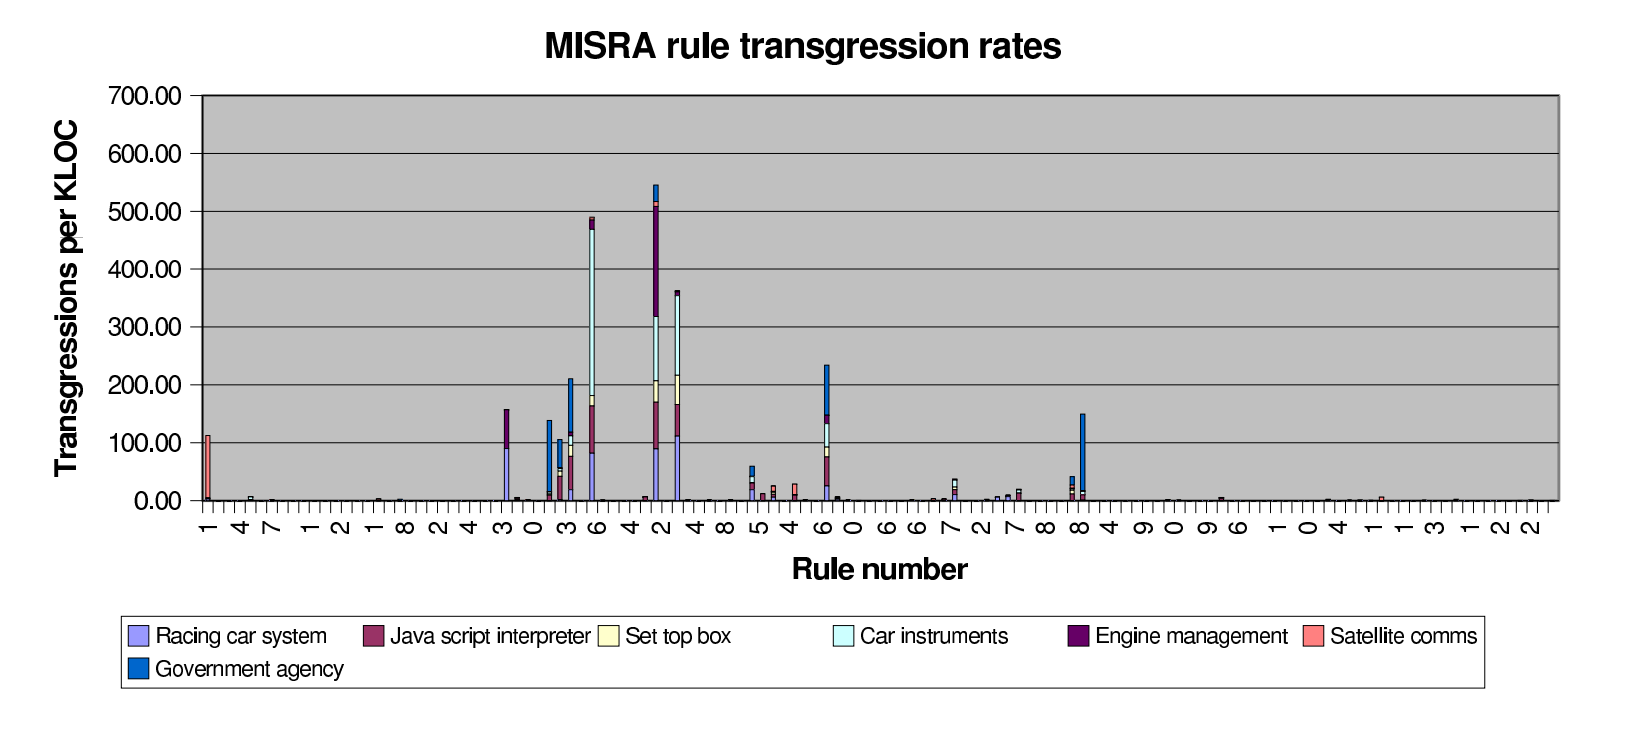
\includegraphics[width=\textwidth]{graphics/2004-transgression-rates.png}
        \caption{Verstöße in Warnungen je 1000 Codezeilen auf 7 Pakete verteilt, M2004\cite{hatton2007language}}
        \label{fig:2004-transgression-rates}
    \end{figure}

    Die Ergebnisse aus~\cite{hatton2007language} sind konsistent mit denen von~\cite{boogerd2008assessing}, welche in
    ihrer Arbeit eine Längsschnittstudie über die Korrelation von Regelverstößen und Faults erstellten.
    Auf Basis des \enquote{TV on Mobile} (TVoM) Projekts der Firma NXP, von dem etwa 91kLoC C Code für die Untersuchung relevant waren.
    TVoM wurde ohne Verwendung von \sqss\ im Allgemeinen bzw.\ \misra\ im Speziellen erstellt.
    Boogerd und Moonen kommen in ihrer Untersuchung zum Schluss, dass 12 von 72 untersuchten Regeln von \misra\ signifikant
    besser als ein zufälliger Prädiktor abschnitten.
    Ihre true positive Raten variierten zwischen 23--100\%.
    Damit handelt es sich bei diesen Regeln um \enquote{gute} Regeln.
    Weiterhin hatten 25 Regeln eine true positive Rate von Null, fanden also keine Faults.
    Zusammen mit den bereits in Abschnitt~\ref{subsec:signal-rausch-rate-und-false-positives} dargelegten Beobachtungen zum
    Rauschen kommen Boogerd und Moonen in Überstimmung mit Hatton zum Schluss, dass die Befolgung des \misra-Standards
    die Qualität der Software wahrscheinlich verschlechtert hätte.
    Die dargebrachten Untersuchungen legten jedoch nur eine Korrelation dar, keinen Kausalzusammenhang.
    Die Beobachtungen könnten sich bei weiteren zu untersuchenden Projekten von den bisherigen unterscheiden.

    \section{Konklusion}
    \label{sec:konklusion}


    %%
    %% Bibliography
    %%

    %% Please use bibtex,

    \bibliography{prosem}

\end{document}
